\documentclass[tikz,border=8pt]{standalone}
\usepackage{amsmath,amssymb}
\usetikzlibrary{arrows.meta,calc,decorations.pathreplacing,patterns,shapes.geometric,positioning,shadings,decorations.pathmorphing}

\begin{document}
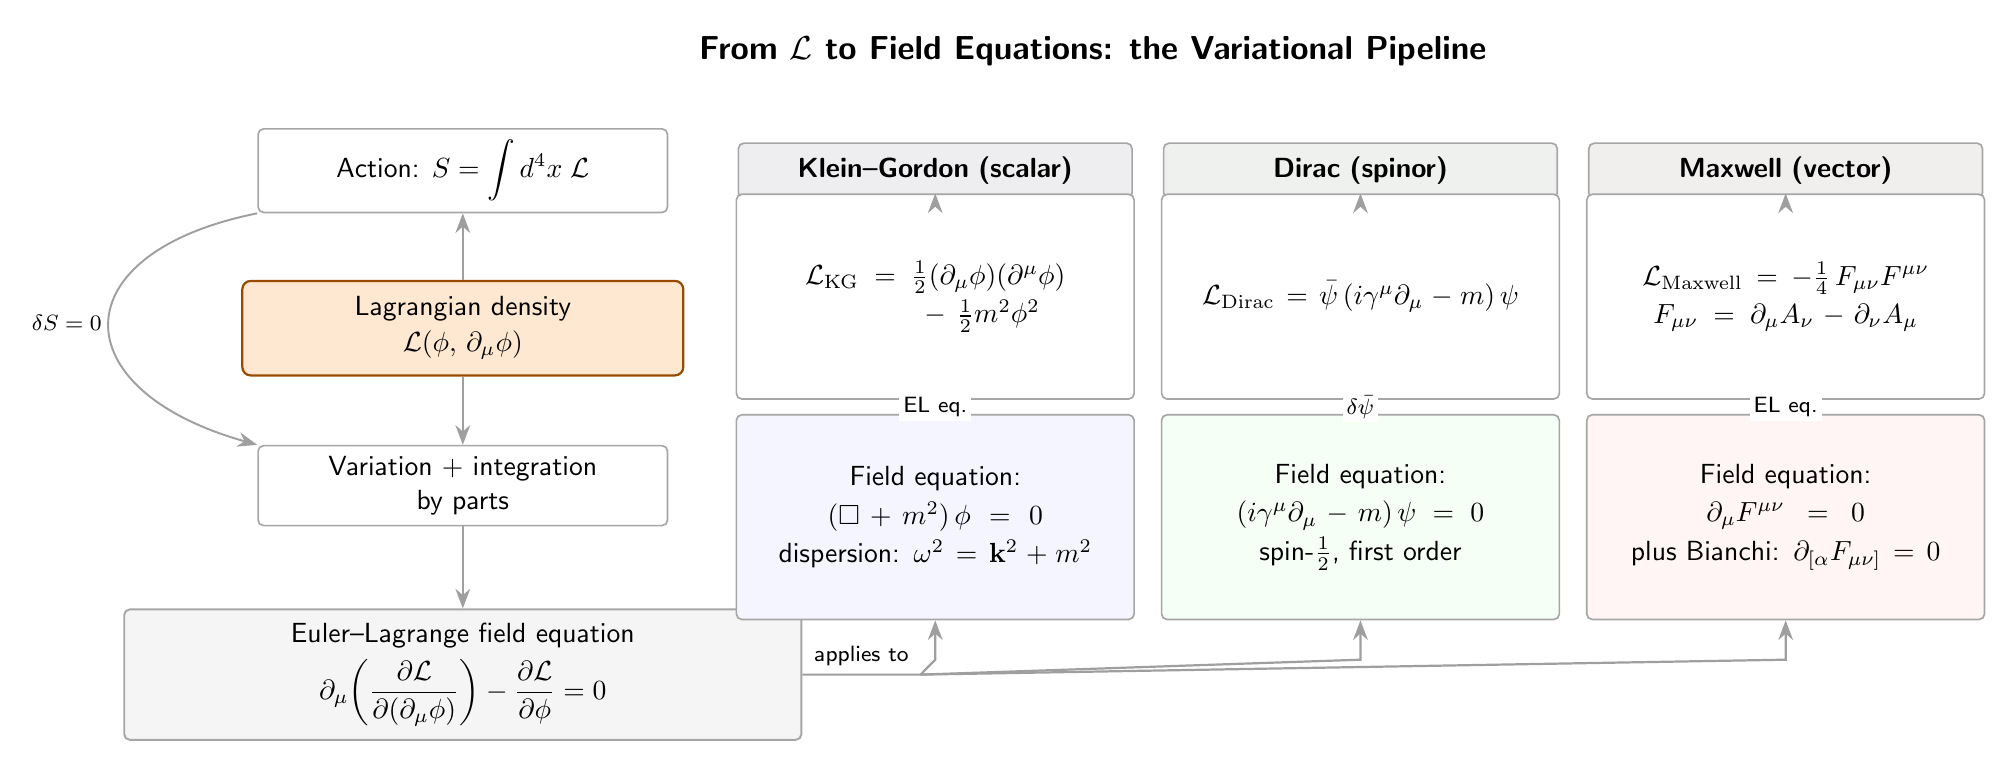
\begin{tikzpicture}[
    font=\sffamily,
    >={Stealth[length=2.5mm]},
    box/.style={rectangle, draw=gray!70, line width=0.6pt, rounded corners=2pt, fill=white, minimum width=5.2cm, minimum height=1.0cm, align=center, inner sep=4pt},
    centerbox/.style={rectangle, draw=orange!60!black, line width=0.8pt, rounded corners=3pt, fill=orange!18, minimum width=5.6cm, minimum height=1.2cm, align=center, inner sep=5pt},
    eqbox/.style={rectangle, draw=gray!70, line width=0.7pt, rounded corners=2pt, fill=gray!8, minimum width=8.6cm, minimum height=1.4cm, align=center, inner sep=5pt},
    examplebox/.style={rectangle, draw=gray!70, line width=0.6pt, rounded corners=2pt, fill=white, minimum width=5.0cm, minimum height=2.6cm, align=center, inner sep=5pt, text width=4.7cm},
    headerbox/.style={rectangle, draw=gray!70, line width=0.6pt, rounded corners=2pt, fill=gray!15, minimum width=5.0cm, minimum height=0.7cm, align=center, inner sep=4pt, text width=4.7cm},
    arr/.style={->, line width=0.7pt, draw=gray!75},
    arrlabel/.style={font=\footnotesize\sffamily, fill=white, inner sep=1.5pt}
]

% --- Left column: pipeline ---
\node[box] (action) at (0, 6.0)
    {Action: $S = \displaystyle\int d^4x \; \mathcal{L}$};

\node[centerbox] (lagr) at (0, 4.0)
    {Lagrangian density\\[1pt] $\mathcal{L}(\phi,\,\partial_\mu\phi)$};

\node[box] (vary) at (0, 2.0)
    {Variation $+$ integration\\ by parts};

\node[eqbox] (el) at (0, -0.4)
    {Euler--Lagrange field equation\\[3pt]
     $\displaystyle \partial_\mu\!\left(\frac{\partial \mathcal{L}}{\partial(\partial_\mu \phi)}\right) - \frac{\partial \mathcal{L}}{\partial \phi} = 0$};

% Arrows in the pipeline
\draw[arr] (lagr.north) -- (action.south);
\draw[arr] (action.south west) .. controls +(-2.5,-0.5) and +(-2.5,0.7) .. node[arrlabel, left=1pt] {$\delta S = 0$} (vary.north west);
\draw[arr] (lagr.south) -- (vary.north);
\draw[arr] (vary.south) -- (el.north);

% --- Right side: three example columns ---
\def\colsep{5.4}
\def\cxA{6.0}
\def\cxB{\cxA+\colsep}
\def\cxC{\cxA+2*\colsep}

\node[headerbox, fill=blue!10!gray!12] (hKG)   at (\cxA, 6.0) {\textbf{Klein--Gordon (scalar)}};
\node[headerbox, fill=green!10!gray!12] (hDir) at (\cxB, 6.0) {\textbf{Dirac (spinor)}};
\node[headerbox, fill=red!10!gray!12] (hMax)   at (\cxC, 6.0) {\textbf{Maxwell (vector)}};

\node[examplebox] (KG) at (\cxA, 4.4)
    {$\mathcal{L}_{\rm KG} = \tfrac{1}{2}(\partial_\mu\phi)(\partial^\mu\phi)$\\[2pt]
     $\hphantom{\mathcal{L}_{\rm KG} = }-\tfrac{1}{2} m^2 \phi^2$};

\node[examplebox] (Dir) at (\cxB, 4.4)
    {$\mathcal{L}_{\rm Dirac} = \bar\psi\,(i\gamma^\mu\partial_\mu - m)\,\psi$};

\node[examplebox] (Max) at (\cxC, 4.4)
    {$\mathcal{L}_{\rm Maxwell} = -\tfrac{1}{4}\, F_{\mu\nu} F^{\mu\nu}$\\[2pt]
     $F_{\mu\nu} = \partial_\mu A_\nu - \partial_\nu A_\mu$};

\node[examplebox, fill=blue!4]  (KGeq)  at (\cxA, 1.6)
    {Field equation:\\[2pt] $(\Box + m^2)\,\phi = 0$\\[2pt]
     dispersion: $\omega^2 = \mathbf{k}^2 + m^2$};

\node[examplebox, fill=green!4] (Direq) at (\cxB, 1.6)
    {Field equation:\\[2pt] $(i\gamma^\mu\partial_\mu - m)\,\psi = 0$\\[2pt]
     spin-$\tfrac{1}{2}$, first order};

\node[examplebox, fill=red!4]   (Maxeq) at (\cxC, 1.6)
    {Field equation:\\[2pt] $\partial_\mu F^{\mu\nu} = 0$\\[2pt]
     plus Bianchi: $\partial_{[\alpha} F_{\mu\nu]} = 0$};

% Arrows from header to L, and L to field equations (vertical, in column)
\draw[arr] (hKG.south)  -- (KG.north);
\draw[arr] (hDir.south) -- (Dir.north);
\draw[arr] (hMax.south) -- (Max.north);

\draw[arr] (KG.south)  -- node[arrlabel] {EL eq.} (KGeq.north);
\draw[arr] (Dir.south) -- node[arrlabel] {$\delta\bar\psi$}  (Direq.north);
\draw[arr] (Max.south) -- node[arrlabel] {EL eq.} (Maxeq.north);

% Arrow from EL central box to the three example columns (forking)
\coordinate (forkstart) at (el.east);
\coordinate (forkmid)   at ($(el.east)+(1.5,0)$);
\draw[arr, line width=0.8pt] (forkstart) -- (forkmid)
    -- ($(KGeq.south) +(0,-0.5)$) -- (KGeq.south);
\draw[arr, line width=0.8pt] (forkmid) -- ($(Direq.south)+(0,-0.5)$) -- (Direq.south);
\draw[arr, line width=0.8pt] (forkmid) -- ($(Maxeq.south)+(0,-0.5)$) -- (Maxeq.south);

% Label on the forking arrow
\node[arrlabel, anchor=south] at ($(forkstart)!0.5!(forkmid) + (0,0.05)$) {applies to};

% Top label / title strip
\node[font=\sffamily\bfseries\large, anchor=south] at (8.0, 7.2)
    {From $\mathcal{L}$ to Field Equations: the Variational Pipeline};

\end{tikzpicture}
\end{document}
